% Introduction

The analysis in this note employs the MNIST Database of Handwritten Digit Images (available online: \url{http://yann.lecun.com/exdb/mnist/}) \cite{lecun1998gradient}. The dataset contains a normalised subset of 70,000 annotated images of handwritten digits collected from the much larger NIST database.
The MNIST dataset modifies instances of handwritten digits in the original NIST database to ensure an equal distribution of instances with respect to the circumstances of data collection.
In particular, the dataset contains an equal number of instances of handwritten digits from collected US census bureaus workers, and from US high school students. In total, 35,000 instances are collected from each category of writer respectively.

Each digit in the dataset is normalised in grey-scale (0-255), and aligned by translating the centre of pixel-mass to be positioned at the centre of a 28x28 pixel grid. 
For the purpose of model estimation, the dataset is partitioned into a training set of 60,000 images, containing equal proportions of instances collected from either category of writer.
The remaining 10,000 instances comprise the test set, and are used for model validation.
Example instances of images from this dataset are presented in Figure \ref{fig:instance-examples}.
The dataset is balanced with respect to the distribution of digit classes (see Figure \ref{fig:class-distributions}).

\begin{figure}
    \caption{Examples of MNIST instances}
	\label{fig:instance-examples}
	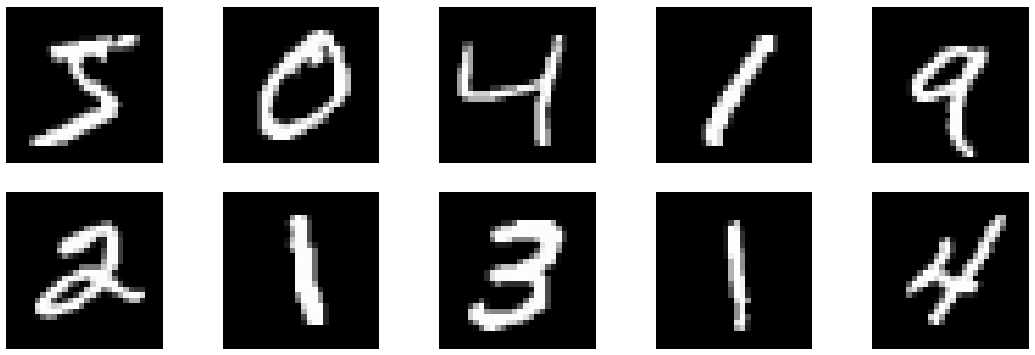
\includegraphics[width=1.0\textwidth]{graphics/instance_examples.pdf}
    \textbf{Notes}: Example instances from the MNIST dataset. Each instance is normalised in grey-scale (0-255), and aligned by translating the centre of pixel-mass to be positioned at the centre of a 28x28 pixel grid. 
\end{figure}

\begin{figure}
    \caption{Distribution of classes in MNIST dataset}
	\label{fig:class-distributions}
	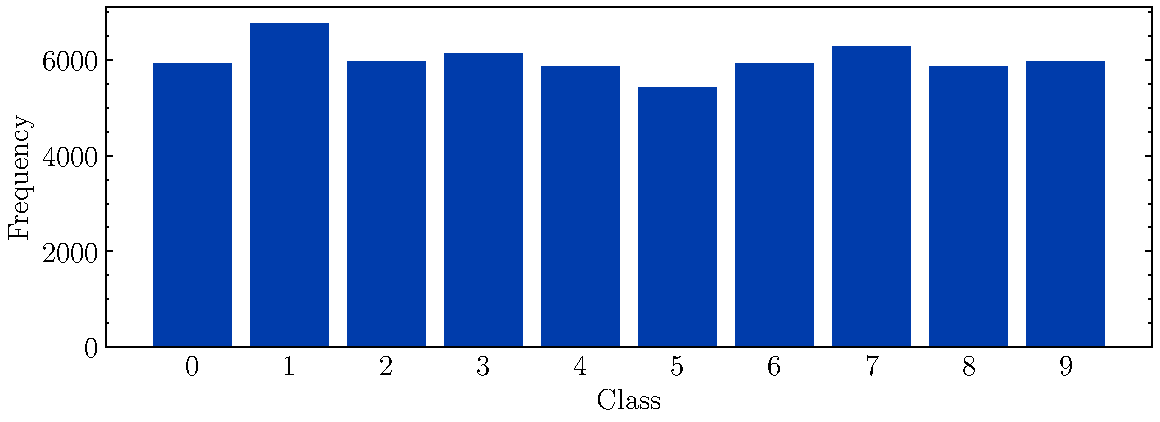
\includegraphics[width=1.0\textwidth]{graphics/class_distribution.pdf}
    \textbf{Notes}: Class distribution of digit instances (0 - 9) in the full MNIST dataset, across both training (N=60,000) and validation (N=10,000) partitions. 
\end{figure}
